\section{Data Link}
The foundation of the entire network stack is the data link layer which
provides reliable bidirectional packet transmission between two nodes in a shared noisy acoustic medium.
The data link layer consists of the physics sublayer and the medium access control sublayer.

\subsection{Physics Sublayer (PHY)}
Bulit on the audio I/O library, PHY enables basic data transmission with no delivery or integrity guarantee.
A PHY frame is a sequence of PCM audio signal samples that represents a chunk of bytes. It is the transmission unit on this layer.
Each frame contains a fixed preamble signal at the beginning for detection as well as synchronization and a payload signal that encodes 0/1 bits.\par
For data transmission, PHY layer constructs a frame from a chunk of bytes and send it through the medium.
For data receiving, PHY layer repeatedly pulls audio samples from the medium and seek for PHY frame based on the frequency-domain feature of the preamble.
When a frame is identified, the payload signal is extracted and decoded.
\subsubsection{Preamble Signal Design}
A chirp is a signal whose instaneous frequency increases or decreases with time.
$x_p(t)$ is a linear chirp signal whose lowest and highest instaneous frequency are $f_a$ and $f_b$ respectively.
\[
	x_p(t) = \begin{cases}
		\pi \dfrac{f_b-f_a}{T} t^2       + 2\pi f_a t     & t\in [0,T]  \\
		\pi \dfrac{f_a-f_a}{T} {(t-T)}^2 + 2\pi f_b (t-T) & t\in [T,2T]
	\end{cases}
\]
Auto-correlation energy peak detection is used to find the starting position of the preamble signal which is followed by the payload signal.

\subsubsection{Modulation and Demodulation}
In order to transmit and receive digital signals, a modulation scheme has to be implemented.
\par
For wireless scenario, strong background noisy is detected from 0Hz to 6000Hz,
so a passband modulation scheme
combining binary phase shift keying (BPSK) and orthogonal frequency-division multiplexing (OFDM)
is implemented.
BPSK encodes bits with phase changes:
\begin{align*}
	x_0(t) & =\sin(2\pi f\, t)
	x_1(t) & =\sin(2\pi f\, t + \pi) = -\sin(2\pi f)
\end{align*}
are used to represent 0 bit and one 1 respectively.
The physics layer sends a bit by pushing samples of the modulated signal to audio I/O driver.
To recover a bit from audio signal, physics layer calculates the dot product of the receive samples and the samples of $x_0(t)$.
\[
	x_0(t)\cdot x_0(t) > 0
	\quad
	x_0(t)\cdot x_1(t) < 0
\]
A zero bit is produced if the dot product is positive, otherwise a one bit is produced.

As for cabel-connected scenario, baseband transmission is possible as low frequency background noise has less power compared with wireless scenario.



\subsubsection{Frame Detection}

\subsection{Medium Access Control sublayer}
\subsubsection{CSMA/CA}
\begin{figure}[h]
	\begin{center}
		\centerline{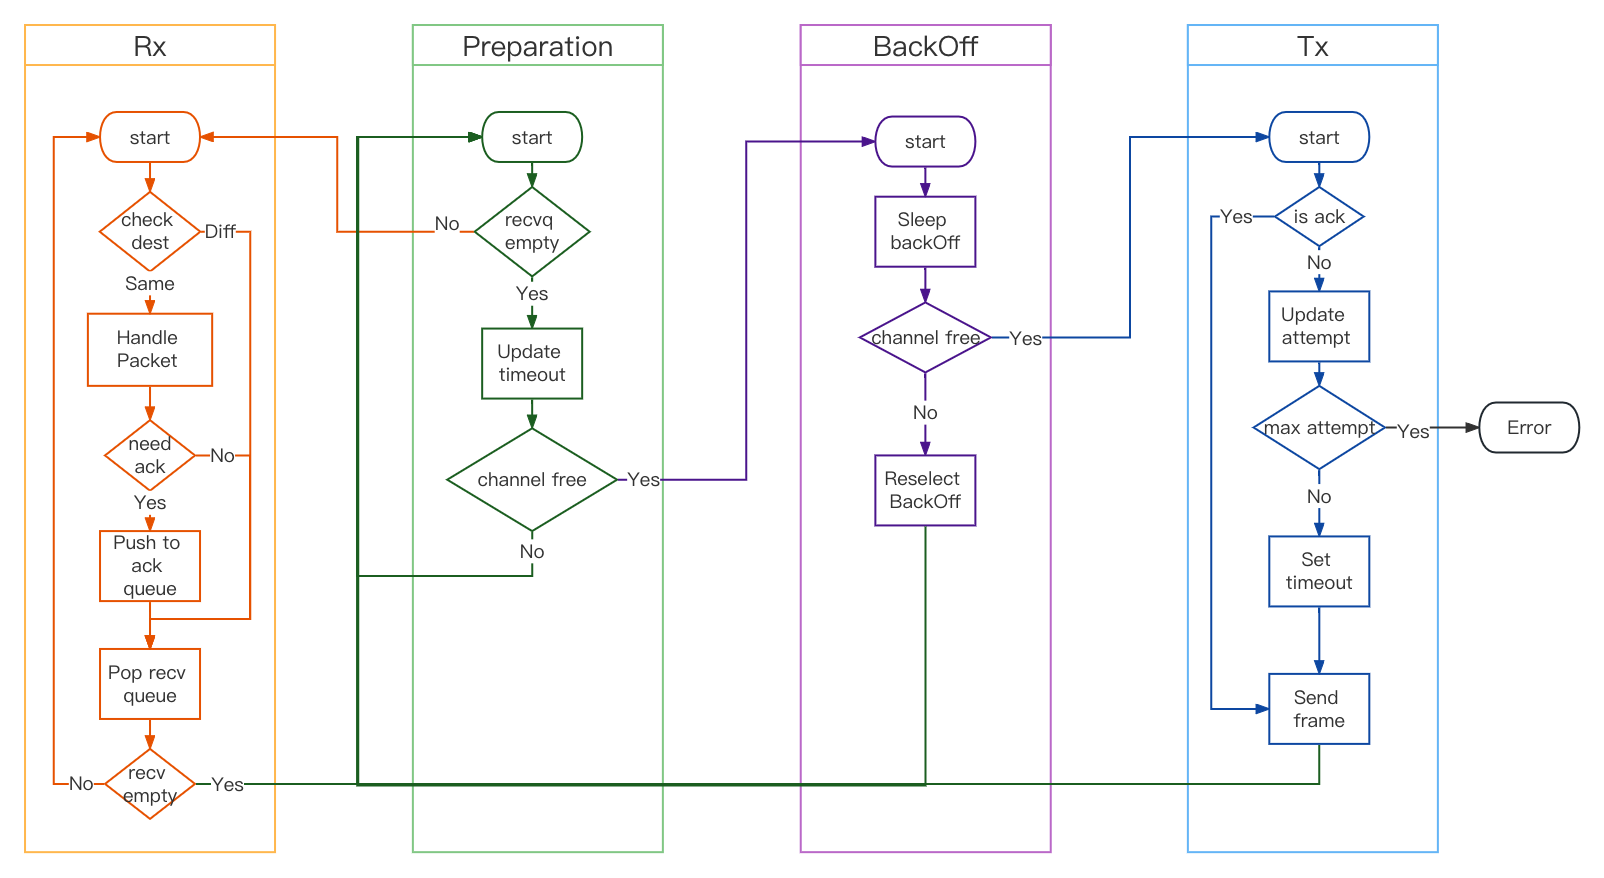
\includegraphics[width=\columnwidth]{./figures/CSMA.png}}
		\caption{the CSMA/CA procdcure}
		\label{csma}
	\end{center}
\end{figure}
The medium access control layer regulates access to the shared medium and retransmission mechanism. Each device will listen to the channel before transmitting. If the channel is busy, the device will wait for a random time and then try to resend the data. The time is chosen by the exponential backoff algorithm. The state transition diagram is shown in Figure~\ref{csma}

\subsubsection{Time-division multiplexing MAC}
Due to the latency of the audio driver, the original CSMA/CA suffers from the remote collision. We also implemented Time-division multiplexing MAC.

\subsection{CSMA}
